\documentclass[twoside, 11pt]{article}
\usepackage[czech]{babel}
\usepackage[a5paper, margin=1.5cm, left = 1.25cm, right = 1.25 cm, bindingoffset=5mm]{geometry}

\usepackage{tgbonum}
\usepackage[T1]{fontenc}



\usepackage{titlesec}


\usepackage{fancyhdr}
\pagestyle{fancy}

\lhead{}
\chead{}
\rhead{}
\cfoot{}
\lfoot{}
\rfoot{\thepage}
\renewcommand{\headrulewidth}{0pt}



\titlespacing*{\section}{0pt}{1.25\baselineskip}{0.25\baselineskip}


\usepackage{wrapfig}

\usepackage{float}
\usepackage{url}
\usepackage{lipsum}
\usepackage[dvipsnames]{xcolor}
\usepackage{anyfontsize}
% \usepackage{showframe}

\usepackage{tikz}
\usetikzlibrary{positioning}

% \usepackage{titlesec}
% \usepackage{fontspec}

% \setmainfont{fbb}
% \newfontfamily\headingfont{Montserrat}

% \titleformat*{\section}{\Large\headingfont}
% \titleformat*{\subsection}{\large\headingfont}
% \titleformat*{\subsubsection}{\headingfont}
\usepackage[labelformat=empty]{caption}
\usepackage{qrcode}

\setlength{\parindent}{0pt}
\setlength{\parskip}{0.5\baselineskip}
% \chead{ \begin{center}
%     \fontsize{40}{43}\selectfont \textcolor{MidnightBlue}{\textbf{NESTRČ!}}
%  \end{center}}

\begin{document}

\addtolength{\topmargin}{-10pt}
\addtolength{\textheight}{10pt}
\headheight = 0pt
\begin{center}
    \fontsize{45}{48}\selectfont \textcolor{MidnightBlue}{\textbf{NESTRČ!}}
 \end{center}


 \begin{tikzpicture}[remember picture,overlay]
    \node [yshift=105.5mm, xshift=2.5mm] (logo) at (current page.center)
        {\color{gray} \rule{\linewidth}{0pt}};
    \node [below=20mm of logo](first)
        {\color{gray} \rule{\linewidth}{1pt}}
        ;
    \node [below=-2mm of first](second)
    {\color{black} \rule{\linewidth}{3pt}}
    ;
    \node [below=-2mm of second](third)
    {\color{gray} \rule{\linewidth}{1pt}}
    ;
\end{tikzpicture}
\vspace{-\baselineskip}
 \large Co? Kam? - Neeee\dots
 \begin{flushright}
    je tu \textcolor{MidnightBlue}{\textbf{Ne}}korektní \textcolor{MidnightBlue}{\textbf{st}}udentský \textcolor{MidnightBlue}{\textbf{r}}ecesistický \textcolor{MidnightBlue}{\textbf{č}}asopis
 \end{flushright}
 \section*{Slovo šéfredaktora:}
 Čau Gevoni, gekoni, pižmoni a jiný mimoni!

 Sem si řek, ž už dobu nevšel žádnej hutnej geváckej plátek (ofikl: školní
 časopis). Tak sem na to sed a upustil trochu páry - hnedle bylo na sjetě pár
 krutě žertovnejch hejtů (rozuměj: satirických článků). Takle má vypadat
 studentskej časák! Žádny krotky recenze a rozhovory vo prdu. Pořádnej
 vodvaz! Tak doufám, ž na mě někdo hnedky naváže a~začnou se házet další
 takovýhle bomby!!! 

 \begin{wrapfigure}[6]{r}{0.25\textwidth}
    \vspace*{-13pt}
    
\includegraphics[width=0.24\textwidth]{funtomas}
    \vspace*{-10pt}
    \begin{flushright}
        \footnotesize{
        \textit{
        \textbf{Váš Funtomas}}}
    \end{flushright}
\end{wrapfigure}

 Dybyste si netroufli rovnou na celý číslo, tak každej suprovej vobrázek,
 námět na článek nebo rovnou hotovej text nasdílejte na mail \mbox{gevotimes@gmail.com} nebo na instagram \mbox{@gevotimes}.
 Posílejte všechny možný nápady, voni si s tim už nějak poraděj\dots

\section*{V tomto čísle:}
Několik skandálních odhalení o Voltovi, Kučerovi a Manuelovi, rozhovor s bývalým profesorem Hodinou, návod jak na prváky, filmové okénko a představení profesorky Dřevojánkové na str. 7.

\clearpage
\headheight = 12pt

\section*{Ethnic friendly v České televizi}
Rada pro rovnoprávné příležitosti před nedávnem
zveřejnila studii vypracovanou komisí odborníků z
ČT a financovanou z grantů EU, MŠMT a MŠ
Jažlovická.


Komise s politováním konstatovala, že po shlédnutí
cca 486 hodin českých večerníčků zjistila, že
pohádky trpí nedostatkem etnické různorodosti.
Téměř všechny hla\-vní večerníčkovské postavy totiž
mají úplně bílou pleť (krom Rákosníčka, který je
překvapivě zelený). Rada ČT se zavázala tento
fatální problém napravit a momentálně se již natáčí
nová verze večerníčkové série Maková panenka a
motýl e-Manuel\dots


\begin{figure}[htbp]
    \centering
    
\includegraphics[width=\textwidth]{emanuel}
\end{figure}
\section*{Aktuálně}
Chuck Norris prý už z Edookitu dokáže zjistit všechno, co potřebuje.

\chead{}
\clearpage
\section*{Kapitalista Volt}
Možná nevíte, že profesor Volt si už před časem založil dodávkovou službu, kterou nazval velmi
originálně, tedy po sobě. Získali jsme výpověď jednoho z pracovníků, kteří rozvážejí nákupy na
motocyklu s krabicí vepředu s nepřehlédnutelným nápisem Wolt:

\uv{Teda, pravda je, že pan Wolt, tedy Volt, nás doslova vykořisťuje! Řek' mi, že abych moh' dobře
vykonávat svou práci a správně kalkulovat zakázky, potřebuju se orientovat v matematice. A
nestačí prý jen sčítání a sem tam nějaký násobení. Je třeba ovládat kvadratické rovnice,
logaritmy a výrokovou logiku. Když jsme se ho ptali, jestli nekecá, odvětil s potměšilým
úsměvem: \uv{Ne, právě naopak!}

A protože většina kurýrů by matematiku na takové úr\-ovni rozhodně nezvládla, nabízel Volt
vychytrale doučování za svou obvyklou taxu 999 Kč/hod. \uv{Vím, není to málo, ale jen si
spočítejte, o kolik více si vyděláte, když zvládnete správně používat diferenciál!}

\begin{figure}[htbp]
    \centering
    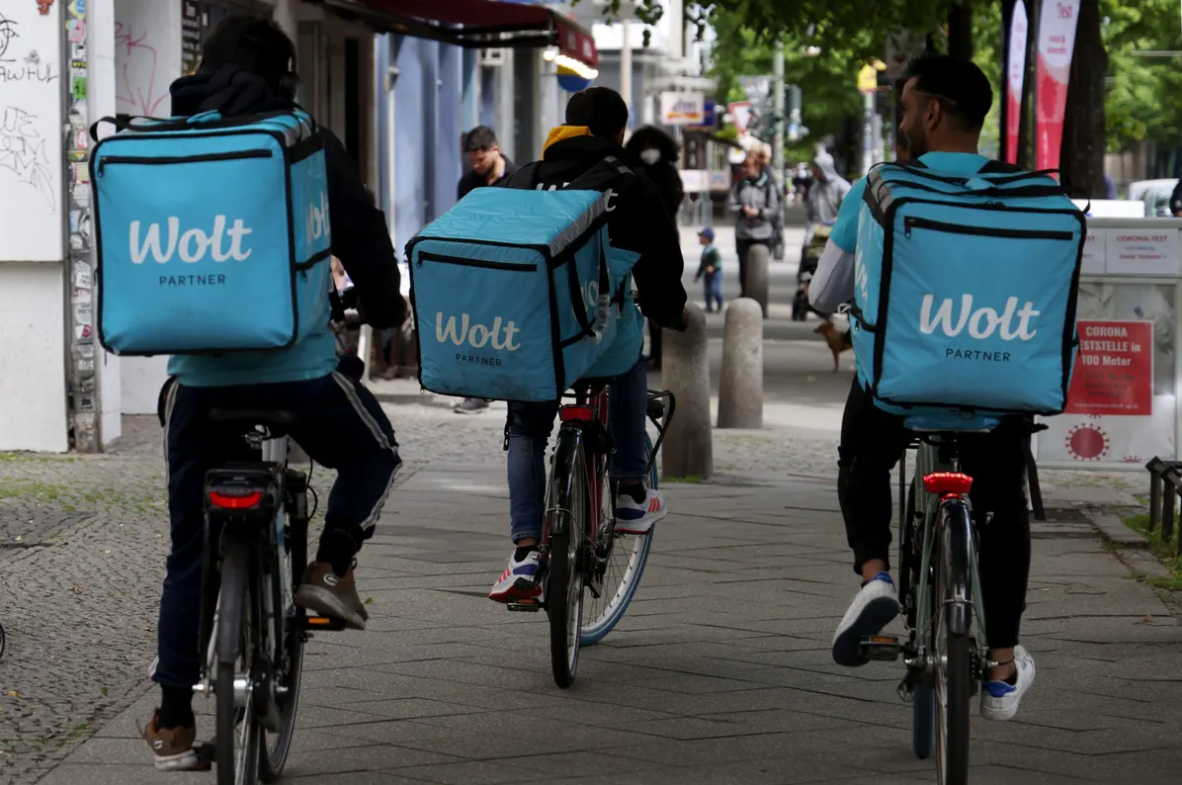
\includegraphics[width=0.7\textwidth]{wolt}
\end{figure}

Bohužel tato osvětová činnost páně profesorově skončila poté, co si jeho nejtalentovanější žák
po roce doučování dokázal spočítat, kolik musí zaměstnavateli měsíčně doplácet, místo toho,
aby vydělával a obětavého Volta mezi kolegy ošklivě pomluvil\dots}
\clearpage

\section*{S Kučertourem mezi mrakodrapy}
Našim reportérům se podařilo získat totálně utajené informace o výjezdu studentů GEVO s prof.
Kučerou do New Yorku. Jeden z účastníků se rozhodl prolomit tabu a promluvit. Poslechněte si
jeho výpověď, pronesenou roztřeseným hlasem:

\uv{Stejně se chci oběsit kvůli tomu testu z fyziky, tak co už\dots \\
Poslouchejte\dots

Pravda je taková, že prof. Kučera vybral od každého přes čtyřicet tisíc na zájezd do NY, trochu
překvapivě ne přes účet školy, ale cash. Jaké bylo naše překvapení, když mikrobus, který nás
měl zavézt na vídeňské letiště, zastavil u poslední benzinky před rakouskými hranicemi a Kučera
místo tankování velel popojet k pestře svítícím neonům nedalekého Casina Imperátor.

\begin{figure}[htbp]
    \centering
    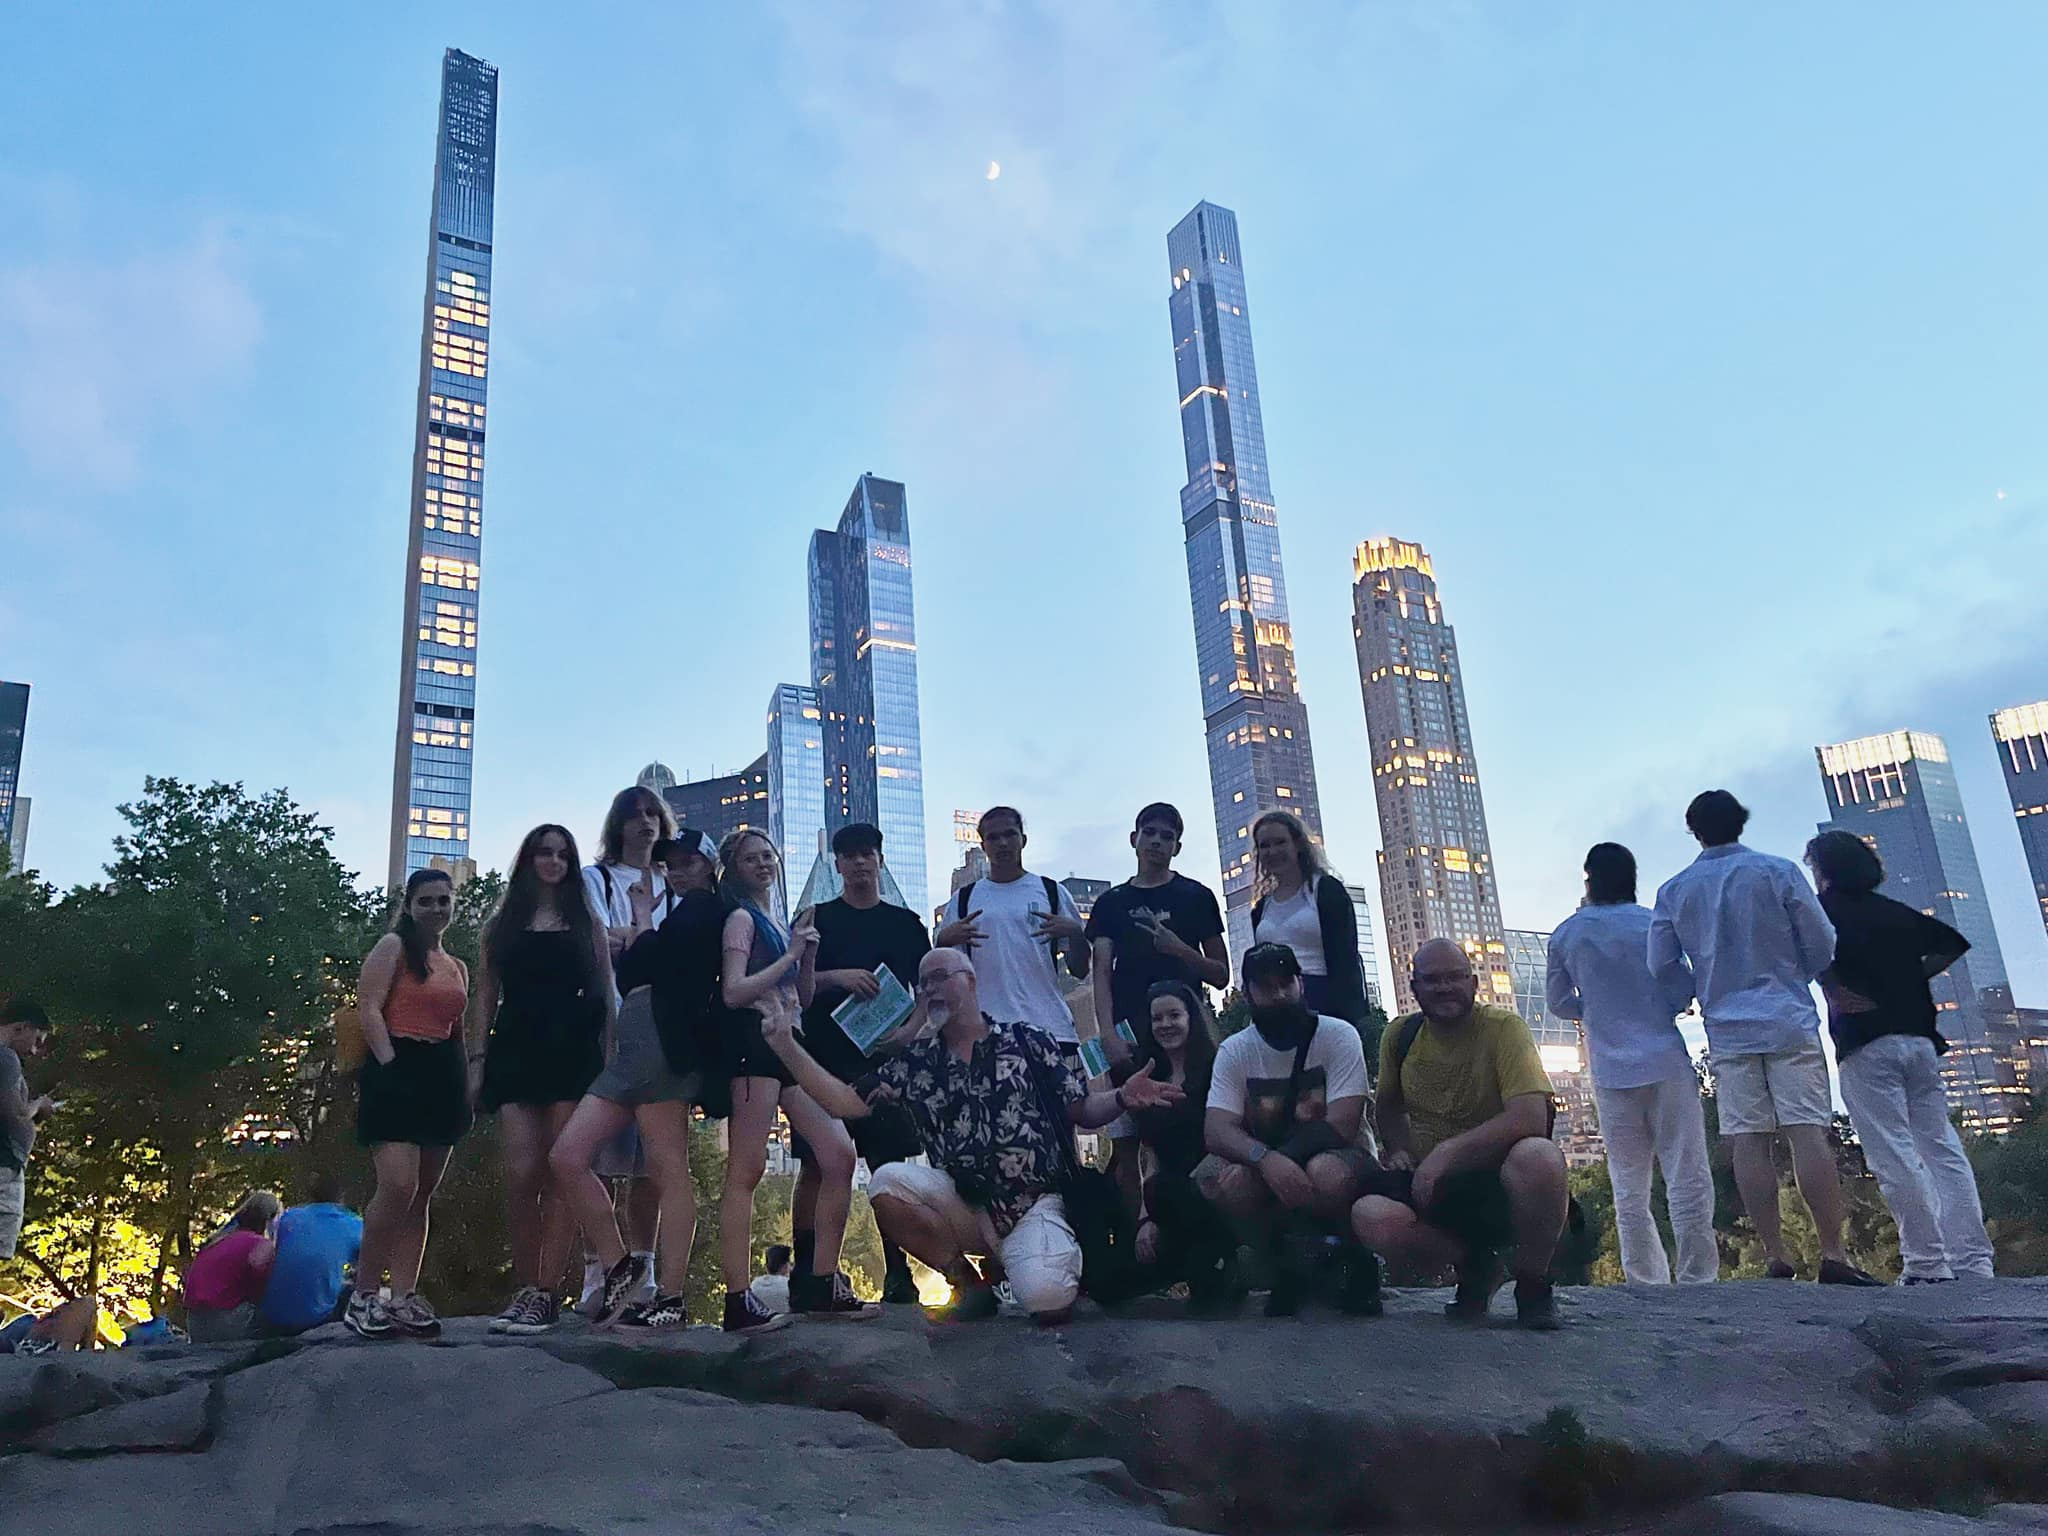
\includegraphics[width=0.62\textwidth]{ny}
\end{figure}

Postavil se před nás a odhodlaně pravil: \uv{Ritz anebo nic!!! Uvědomte si, že s takovýmito penězi
se už dá v~casinu leccos podniknout! Pravda, může se stát, že půjdeme domů pěšky. Ale taky je
možné, že do New Yorku poletíme business class, ubytujeme se v hotelu Plaza, večeřet budeme
chodit do Eleven Madison Park, každá studentka si domů přiveze boty Manolo Blahnik a každý
student tenisky Vans Ultra Limited Edition. - Tak co? Jdeme do toho?}

Oči mu svítily a jeho podmanivý hlas nás paralyzoval jako oběť kobry. Překvapením a údivem
jsme nedokázali ani pípnout, což vedoucí zájezdu pochopil jako souhlas…


Následný pochod domů nám trval přesně týden, přece jenom jsme nebyli navyklí tolik ťapat a
prof. Kučera navíc udělal drobnou zacházku přes Brno, kde stojí rekordní výšková budova v ČR.
Cesta nám příjemně ubíhala, neboť pedagog celou dobu živě vyprávěl o mrakodrapech New
Yorku a uměleckých dílech z tamních galérií, abychom měli co doma o zájezdu vyprávět.
Samozřejmě také vyslovil jisté hrozby na adresu toho, kdo by porušil mlčenlivost. U zeleně
natřené boudy venkovních záchodků benzinky v Průhonicích ještě Kučera pořídil několik
skupinových fotografií, aby tam na pozadí mohl naklíčovat mrakodrapy a poslat obrázky
rozesmátých studentů v New Yorku Bížovi na FB. A to je všechno. Teď víte pravdu!}

Těmito slovy se s námi dotyčný student rozloučil a odešel na Opatov skočit pod vlak.

\section*{Filmový propadák léta 2023}
O čem bude řeč? Napoví tento obrázek:

\begin{figure}[htbp]
    \centering
    
\includegraphics[width=0.9\textwidth]{barbie}
\end{figure}
\vspace*{-12pt}
{\scriptsize Ano správně, jde o absolutní výbuch Kazmova filmu Onemanshow, který sice první týden přilákal do kin rekordní počet návštěvníků, ale divácky totálně propadl již čtvrtý týden po premiéře. Svědčí to o něčem? - Samozřejmě, že ano. (Ale o čem???)}
\clearpage

\section*{Zpověď}
(rozhovor s nyní již bývalým profesorem hudby \textbf{Jiřím Hodinou})

\begin{wrapfigure}[10]{r}{0.35\textwidth}
    \vspace*{-4pt}
    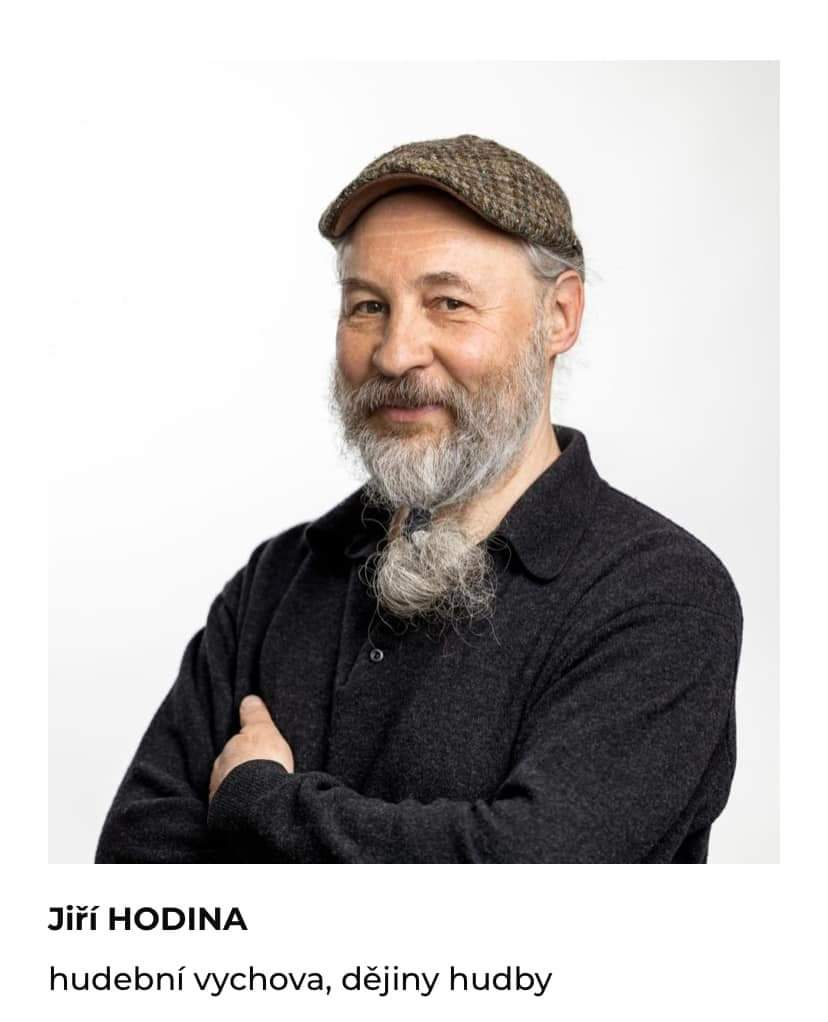
\includegraphics[width=0.34\textwidth]{hodina}
\end{wrapfigure}


Štábu naší redakce se \textbf{před hodinou} podařilo zjistit šokující novinku:
\textbf{prof. Hodina} byl v červnu ředitelem školy \textbf{na hodinu} propuštěn.
Sám perzekuovaný pedagog nám k tomu řekl: \uv{Byla to pro mne opravdu
\textbf{těžká hodina}, ale nakonec se mi ulevilo, protože jsem právě otevřel síť
\textbf{hodinových hotelů} a na nějaké \textbf{hodiny hudební výchovy} bych už
neměl \textbf{ani minutu}\dots}

\section*{Poradna}
\textbf{Co říct prvákům, aby konečně drželi zobák}\\ aneb \textbf{Tak to je krutý!}
  
\begin{itemize}
    \item Tvůj králíček umřel, protože tě už opravdu nesnášel.
    \item To, co máš na tváři, ve skutečnosti nejsou pihy, ale stopy od špinavých myší, které ti v noci přebíhají po obličeji.
    \item Paní kuchařce v jídelně prý spadla do hrnce zubní protéza. Kdo jí najde v jídle, má jí
    odevzdat do kanceláře.
    \item Tví rodiče mě pověřili, abych ti nějak šetrně sdělil, že jsi adoptovaný\dots Co? Jak, kdo jsou
    teda tví praví rodiče??? No přece vaši! - Ti noví, co tě adoptovali, si pro tebe přijdou dnes
    po obědě ke gymplu\dots
    \item Mluvící papoušci, jako je třeba Čenda, byli kdysi studenty.
    V papoušky je proměnila zlá víla, která je přistihla při
    onanování.
    \item Jo a víš, jak se dělají tví oblíbení gumoví medvídci? Jsou
    to ve skutečnosti hovínka od těch pestrobarevných
    papoušků, co dřív bývali studenty.
    \item Učitelé začali stávkovat\dots ~Ale neboj, soukromých škol se
    to netýká.
    \item Až zase půjdeš při hodině na záchod, tak nezapomeň, že neteče voda! Chodí se do křoví
    před školou - kluci vlevo, holky vpravo. Utírá se listím.
    \item Klid! Kdo dostal z testu za pět, ten si to opraví, protože ho profesor hned příští hodinu
    vyvolá, aby ho u tabule před třídou vyzkoušel.
    \item Říkáme ti sice Honzo, ale ve skutečnosti se jmenuješ RX300-87MkII a rodiče tě koupili
    v Lidlu.
    \item Nepamatuješ si vzorečky? Tak si je odvoď, ne?
\end{itemize}

\section*{Představení profesorky Dřevojánkové:}
TO JE VONA\dots \\
\begin{wrapfigure}[3]{r}{0.35\textwidth}
    \vspace*{-40pt}
    
\includegraphics[width=0.34\textwidth]{libiak}
\end{wrapfigure}

A jestli si myslíte, že je to Libiaková, tak se šeredně pletete!
\vfill
\begin{flushright}
    - Cha cháá, teď bude muset několikrát denně říkat -ř  
\end{flushright}

\clearpage

\begin{center}
    \Large \textbf{Hledáme kreslíře a karikaturisty!!!}
\end{center}

\begin{center}
    \Large \textbf{Soutěž o nejlepší podobiznu některého z~profesorů či profesorek - kdo máte jakoukoliv kresbičku, pošlete ji!}
\end{center}
\centering

\includegraphics[width=0.97\textwidth]{wanted}

\lfoot{\scriptsize Obrázky zasílejte na: gevotimes@gmail.com nebo na instagram @gevotimes}
\end{document}
